\section{Failure Recovery and Qualitative Diagnostics}
\label{sec:failure-qualitative}

Qualitative evidence is most useful when organized by a mechanism and tied to
scene-level metrics.  We therefore analyze the fixed hard set first, then give
traceable examples of recovered, persistent, and newly introduced failures.
All quantitative hard-set results and the mechanism-organized case table use
the same historical checkpoint pair as the main paper's 367-versus-440
recovery claim.  The final full-benchmark visualization is separately labeled
and is not used in the 658-scene recovery analysis.

\subsection{Construction of the fixed 658-scene set}
\label{sec:hard658}

The set contains 658 NAVSIM v1 scenes for which the initial ReCogDrive policy
obtained exactly zero PDMS in all five construction samples because of an
at-fault collision (NC), drivable-area violation (DAC), or both.  The set is
fixed before comparing the scalar-GRPO and AMPT recovery checkpoints.  Under
single-trajectory evaluation, scalar GRPO is positive on 367 and zero on 291
scenes; the AMPT recovery checkpoint is positive on 440 and zero on 218.

The paired $2\times2$ transition is
\begin{equation}
\begin{array}{c|cc|c}
 & \multicolumn{2}{c|}{\text{AMPT recovery checkpoint}} & \\
\text{scalar GRPO} & \text{zero} & \text{positive} & \text{row total} \\
\hline
\text{zero}     & 198 & 93  & 291 \\
\text{positive} & 20  & 347 & 367 \\
\hline
\text{column total} & 218 & 440 & 658
\end{array}.
\label{eq:hard658-transition}
\end{equation}
Hence 93 failures are repaired, 347 successes are retained, 198 failures
persist, and 20 new failures appear.  The net change is $93-20=73$, exactly the
difference between the gross positive counts $440-367$.  This distinction is
important: 440/658 is the gross recovery rate relative to the policy used to
construct the hard set, whereas 93 and 20 describe the paired transition from
scalar GRPO to the AMPT recovery checkpoint.  The resulting 11.1-percentage-
point paired improvement has a scene-bootstrap 95\% CI of 8.1--14.3 points
(10,000 resamples, seed 2027).  It is a net improvement rather than an exchange
of an equal number of old and new failures.

\begin{table}[t]
\centering
\small
\caption{Recovery on the same 658 NAVSIM v1 scenes under one archived comparison. Rates use Wilson 95\% intervals over scenes; this interval does not represent training-seed uncertainty. Higher recovery is better.}
\label{tab:failure_recovery}
\resizebox{\linewidth}{!}{%
\begin{tabular}{lcccccc}
\toprule
Method & Positive & Zero & Recovery rate (\%) & Wilson 95\% CI (\%) & Runs & Scenes \\
\midrule
Scalar GRPO & 367 & 291 & 55.8 & [52.0, 59.5] & 1 archived comparison & 658 \\
AMPT recovery checkpoint & 440 & 218 & 66.9 & [63.2, 70.4] & 1 archived comparison & 658 \\
\bottomrule
\end{tabular}%
}
\end{table}

\begin{table}[t]
\centering
\small
\caption{Paired recovery change on 658 NAVSIM v1 scenes. The 11.1-point gain has a scene-paired bootstrap interval (10,000 resamples, analysis seed 2027); higher net repair is better. One archived model pair is available.}
\label{tab:failure_net_gain}
\resizebox{\linewidth}{!}{%
\begin{tabular}{lcccccc}
\toprule
Absolute gain (pp) & Paired 95\% CI (pp) & Zero-to-positive & Positive-to-zero & Net repair & Scenes & Runs \\
\midrule
11.1 & [8.1, 14.3] & 93 & 20 & 73 & 658 & 1 archived comparison \\
\bottomrule
\end{tabular}%
}
\end{table}


\begin{figure}[t]
  \centering
  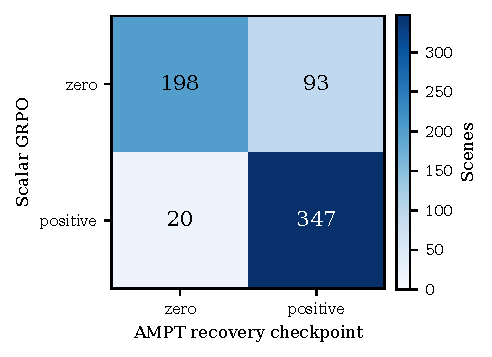
\includegraphics[width=\linewidth]{figures/generated/failure_transition.pdf}
  \caption{Scalar-GRPO to AMPT transition on the fixed 658-scene set.  The
  off-diagonal cells expose both 93 repairs and 20 regressions, rather than
  reporting gross recovery alone.}
  \label{fig:failure-transition}
\end{figure}

The original hard-set taxonomy contains 480 DAC-only scenes, 165 collision-
only scenes, 13 scenes failing both, and no residual ``other'' category.  The
paired repairs/new failures are 59/14 for DAC-only, 32/6 for collision-only,
and 2/0 for the joint category, giving net changes of 45, 26, and 2 scenes.
The gains are therefore not concentrated in only one failure type, although
the small joint category is descriptive rather than statistically decisive.

\begin{table}[t]
\centering
\small
\caption{Failure-type decomposition for the fixed 658 NAVSIM v1 scenes. Repairs and regressions use the scalar-GRPO to AMPT transition; net repairs sum to 73. One archived comparison; higher net repair is better.}
\label{tab:failure_causes}
\resizebox{\linewidth}{!}{%
\begin{tabular}{lcccc}
\toprule
Failure type & Scenes & Repairs & Regressions & Net repair \\
\midrule
DAC-only/all-fail & 480 & 59 & 14 & 45 \\
collision-only/all-fail & 165 & 32 & 6 & 26 \\
collision + DAC & 13 & 2 & 0 & 2 \\
\bottomrule
\end{tabular}%
}
\end{table}


\begin{figure}[t]
  \centering
  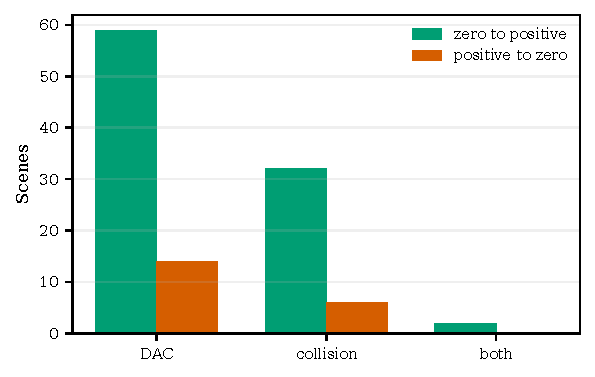
\includegraphics[width=\linewidth]{figures/generated/failure_cause_recovery.pdf}
  \caption{Repairs and regressions by the fixed hard-set cause taxonomy.  The
  net changes are 45 DAC, 26 collision, and 2 joint cases, totaling 73.}
  \label{fig:failure-causes}
\end{figure}

\subsection{Traceable scene cases}
\label{sec:traceable-cases}

Table~\ref{tab:hard658-cases} selects cases by transition type, not by visual
appeal.  Navigation commands come from the corresponding NAVSIM scene
metadata; scores and components come from the fixed paired evaluation.  The
table uses full scene identifiers so every row can be regenerated.  Component
pairs are scalar-GRPO $\rightarrow$ AMPT-recovery values.

\begin{table*}[t]
\centering
\small
\caption{Mechanism-organized examples from the fixed 658-scene set. Scene IDs and PDMS values are reproduced from the archived comparison; commands are joined from audited scene metadata. These selected cases are not an unbiased benchmark sample.}
\label{tab:hard658-cases}
\resizebox{\textwidth}{!}{%
\begin{tabular}{lccccccccc}
\toprule
Scene ID & Command & Outcome & PDMS & NC & DAC & TTC & EP & DDC & Diagnosis \\
\midrule
00fcad6d092c5e8e & left & repaired & 0.000 -> 1.000 & 0.000 -> 1.000 & 1.000 -> 1.000 & 0.000 -> 1.000 & 0.000 -> 1.000 & 1.000 -> 1.000 & Collision/TTC failure repaired without protected regression. \\
03aa8a0576a25b63 & right & repaired & 0.000 -> 0.963 & 1.000 -> 1.000 & 0.000 -> 1.000 & 1.000 -> 1.000 & 0.000 -> 0.912 & 1.000 -> 1.000 & Drivable-area failure repaired while NC and TTC remain feasible. \\
1148c72f141c532d & left & partial repair & 0.000 -> 0.583 & 0.000 -> 1.000 & 0.000 -> 1.000 & 0.000 -> 0.000 & 0.000 -> 1.000 & 1.000 -> 1.000 & Both hard failures repaired; TTC remains the limiting component. \\
00016f8b45c25a1d & left & persistent & 0.000 -> 0.000 & 1.000 -> 1.000 & 0.000 -> 0.000 & 1.000 -> 1.000 & 0.000 -> 0.000 & 0.000 -> 0.000 & DAC/progress failure persists under both audited checkpoints. \\
4b4a268bee4c5ab5 & left & regressed & 1.000 -> 0.000 & 1.000 -> 1.000 & 1.000 -> 0.000 & 1.000 -> 1.000 & 1.000 -> 0.000 & 1.000 -> 1.000 & A DAC regression creates a new zero and motivates retention. \\
\bottomrule
\end{tabular}%
}
\end{table*}


The first two cases are consistent with feasibility-oriented recovery: a hard
component changes from zero to one and positive PDMS returns.  Scene-level
before/after metrics do not identify the temporal order of training updates.
The third shows why ``recovered'' does not mean component-wise perfect.  The
fourth remains a DAC/progress failure under both audited checkpoints; without a
candidate/rollout manifest, the metrics do not identify whether pool coverage,
policy support, or optimization is responsible.  The fifth prevents
survivorship bias in the qualitative analysis and
motivates APR retention; it is one of the 20 positive-to-zero transitions
already charged against net recovery.

\subsection{Mechanism-centered visualization protocol}
\label{sec:qualitative-protocol}

The supplied renderer groups panels by decision rather than by scene
similarity.  A PC-MTS panel overlays an accepted candidate, a rejected distant
candidate, the logged trajectory, and the frozen-policy rollout neighborhood.
An FF-PGRPO mixed-group panel distinguishes unsafe, feasible-but-dominated,
and admissible Pareto-positive rollouts and prints their assigned advantages;
an all-infeasible panel shows the coherent recovery reference.  An APR panel
shows the current prediction, raw teacher, evaluated interpolant, and the
accepted/expired/newly-activated lifecycle state.  Every rendered panel reads
the scene id, command, component scores, and method name from its manifest and
uses a common legend: blue for the current prediction, green for an accepted
or positively credited trajectory, orange for a dominated/expired trajectory,
red for an unsafe trajectory, and black dashed for the coherent reference.

This protocol is also a safeguard against overinterpretation.  A camera/BEV
image is emitted only when the frame, command, all trajectories, and evaluator
record share the same scene identifier.  The metric-only cases in
Table~\ref{tab:hard658-cases} remain quantitative case studies if those visual
assets are unavailable; no unrelated camera frame or hand-drawn trajectory is
substituted merely to complete a panel.

\begin{figure*}[t]
  \centering
  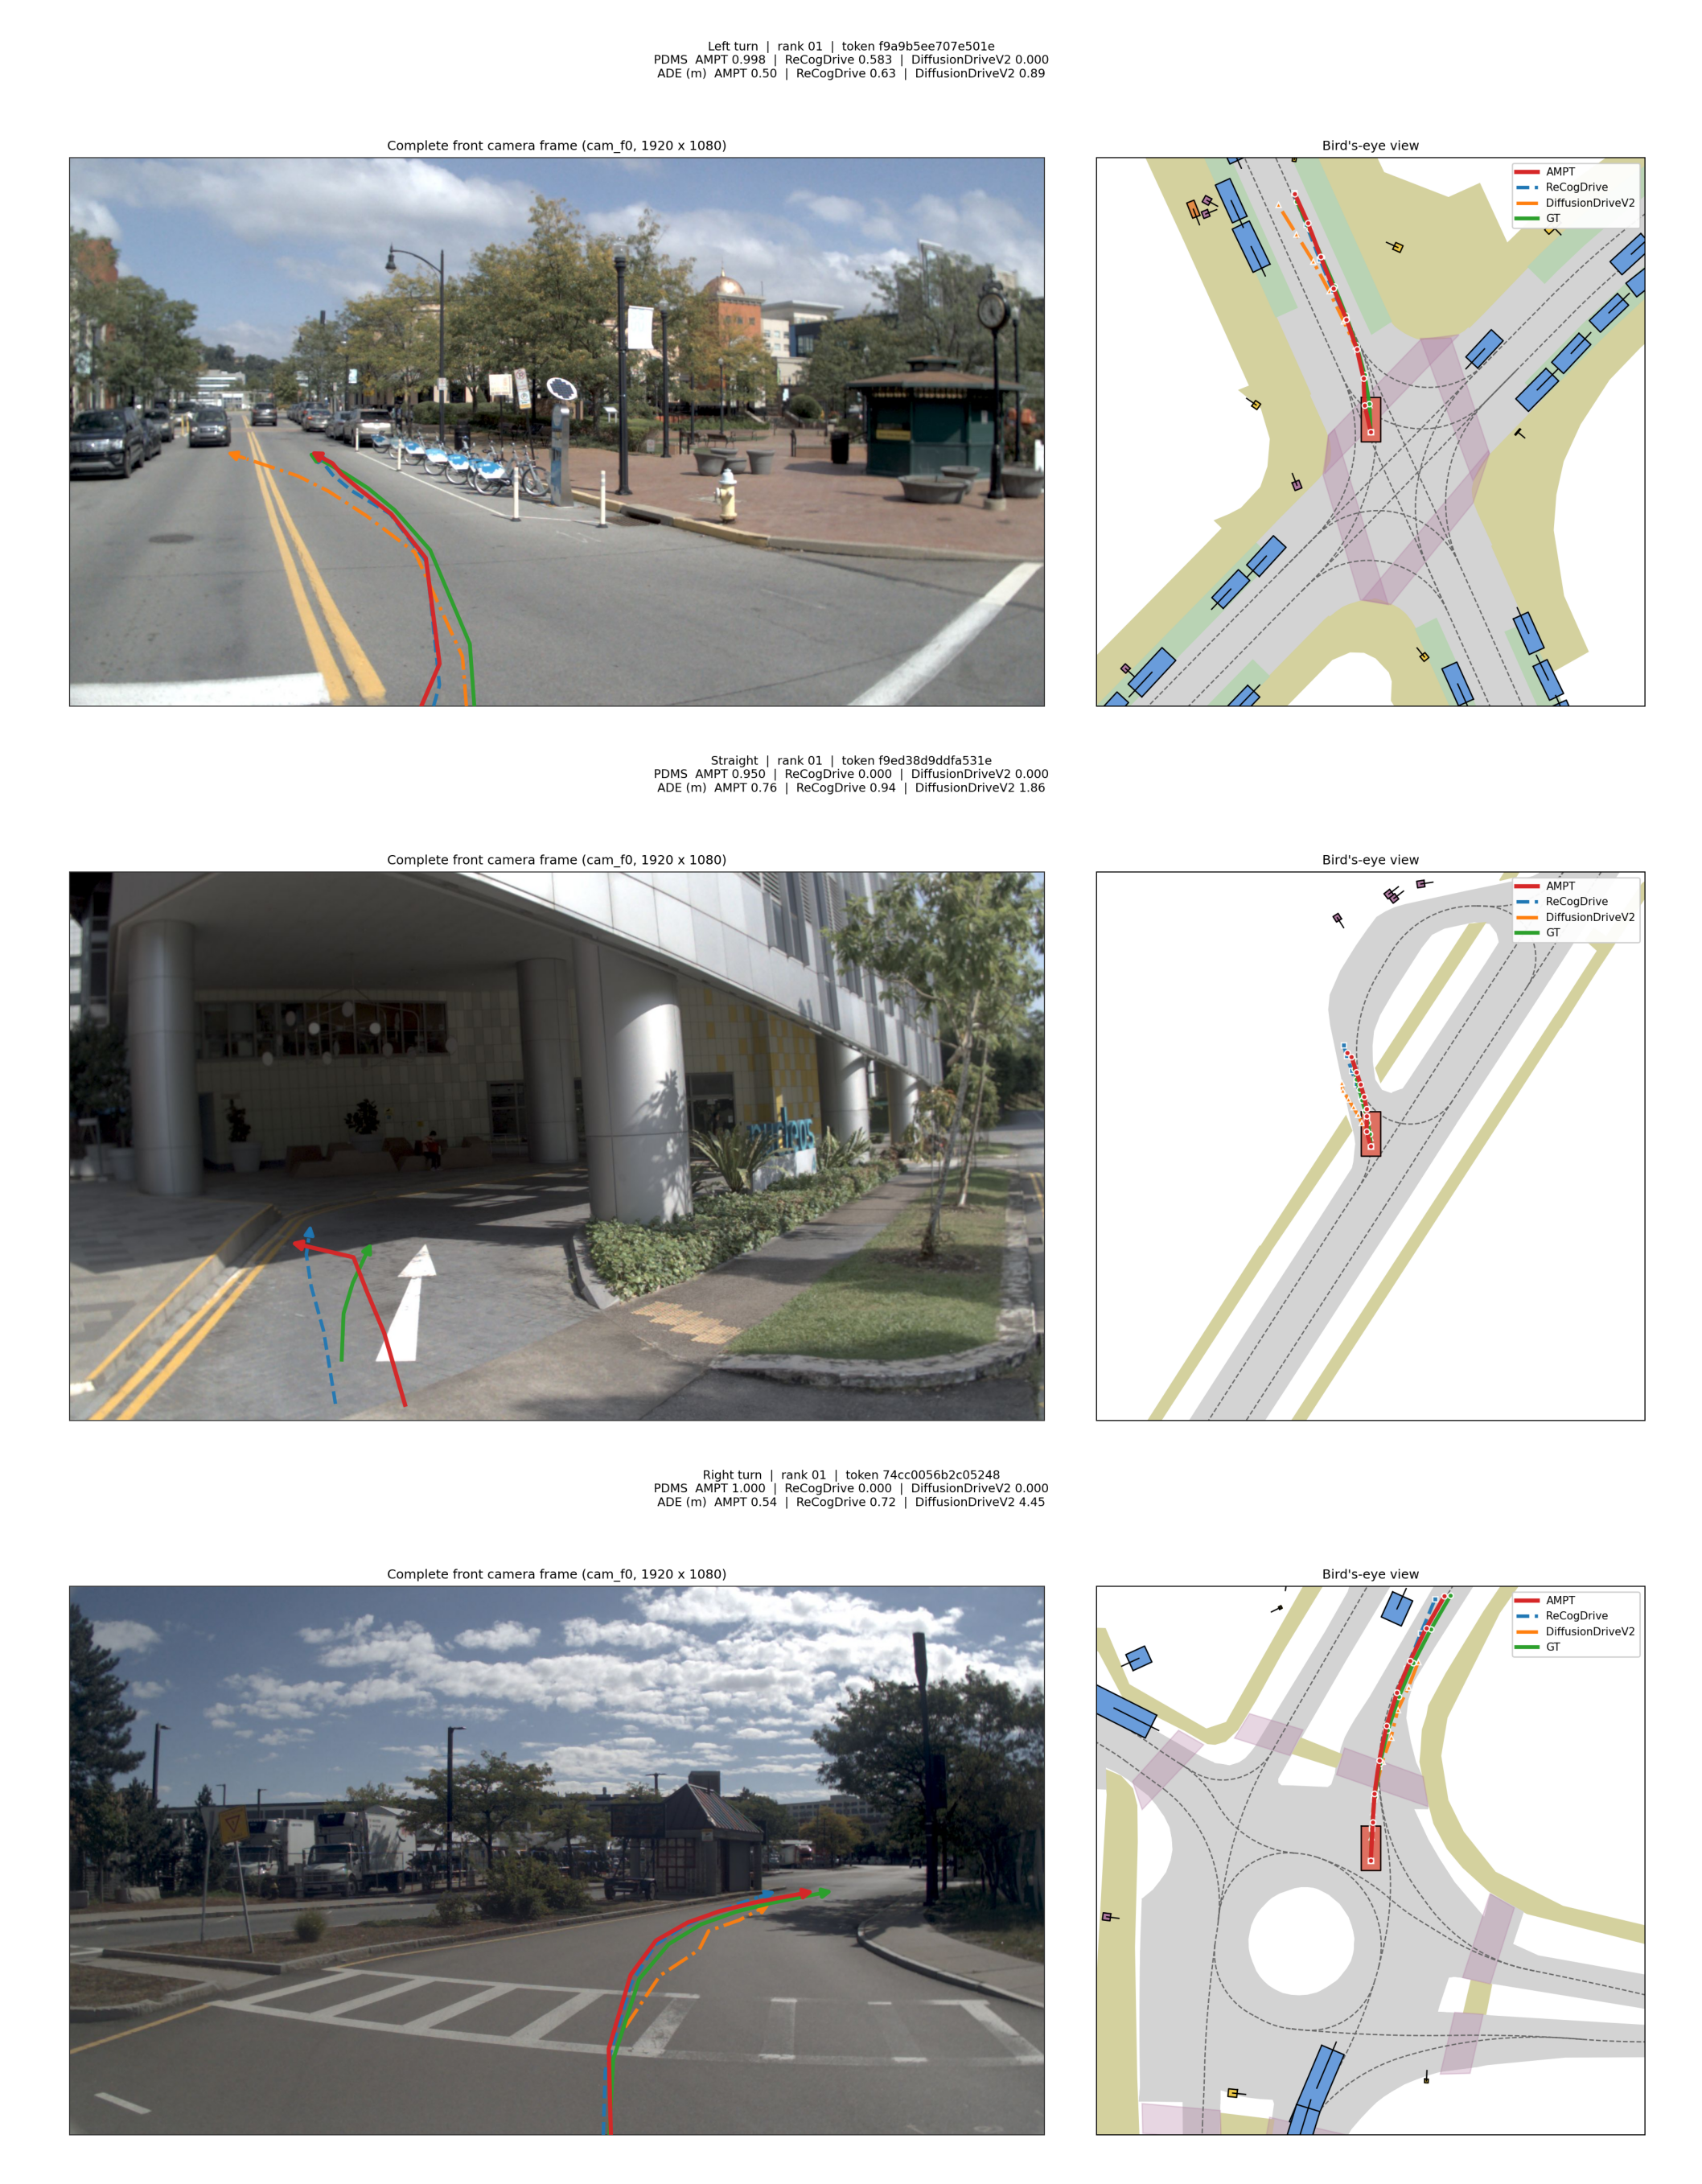
\includegraphics[width=0.92\textwidth]{figures/generated/qualitative_selected_cases.png}
  \caption{Three selected full-benchmark NAVSIM v1 cases (left, straight, and
  right commands) rendered from the separately audited final-AMPT manifest.
  Each row contains the complete front frame, bird's-eye view, scene ID,
  command, color legend, PDMS, and trajectory error.  These examples are not
  members of, and contribute no statistics to, the historical 658-scene
  recovery comparison; they illustrate final-policy behavior only.}
  \label{fig:qualitative-selected}
\end{figure*}

\clearpage
